\documentclass[12pt]{report}
\setcounter{tocdepth}{5}
\setcounter{secnumdepth}{5}
\usepackage{geometry}
\geometry{a4paper}

%%% PACKAGES
\usepackage{booktabs} % for much better looking tables
\usepackage{array} % for better arrays (eg matrices) in maths
\usepackage{enumitem} % very flexible & customisable lists (eg. enumerate/itemize, etc.)
\usepackage{spverbatim} % adds environment for commenting out blocks of text & for better verbatim
\usepackage{subfig} % make it possible to include more than one captioned figure/table in a single float
%\usepackage[ngerman]{babel} % German umlauts
%\usepackage[T1]{fontenc}
\usepackage{lmodern} % fancy fonts for PDF(Reader)
\usepackage{graphicx} % show graphics
\usepackage{listings} % Sourcecode
\usepackage{color}
\usepackage{courier}
\usepackage{nameref}
\usepackage{lastpage}
\usepackage{hyphenat}
\usepackage{textcomp}
\usepackage{float}
\usepackage[section]{placeins}
\usepackage{pbox}
\usepackage{amsmath}
\usepackage{MnSymbol}
\usepackage{wasysym}
\usepackage{parskip}
\usepackage{pifont}
\usepackage{pdfpages}
\usepackage{longtable}
\usepackage[table]{xcolor}
\usepackage{fancyvrb}

\usepackage[defaultlines=4,all]{nowidow}
\setnoclub[3]
\setnowidow[3]

\definecolor{tudogreen}{RGB}{132,184,24}
\definecolor{TUDOGREEN}{RGB}{132,184,24}
\definecolor{tudogreen10}{RGB}{243,248,232}
\definecolor{tudogreen30}{RGB}{218,234,186}
\definecolor{tudogray10}{RGB}{236,236,236}
\definecolor{tudogray20}{RGB}{218,218,218}
\definecolor{tudogray40}{RGB}{102,102,102}
%\input{xtra-tudo-color.tex}
%\input{xtra-tex-command.tex}

\AtBeginDocument{\renewcommand\contentsname{\textcolor{tudogreen}{Table Of Contents}}}

\usepackage{sectsty}
\chapterfont{\color{tudogreen} \hypersetup{linkcolor=tudogreen}}
\sectionfont{\color{tudogreen} \hypersetup{linkcolor=tudogreen}}
\subsectionfont{\color{tudogreen} \hypersetup{linkcolor=tudogreen}}
\subsubsectionfont{\color{tudogreen} \hypersetup{linkcolor=tudogreen}}
\paragraphfont{\color{tudogreen}}
\let\oldparagraph\paragraph\renewcommand{\paragraph}[1]{\oldparagraph{#1}\mbox{}\\}
\subparagraphfont{\color{tudogreen}}
\let\oldsubparagraph\subparagraph\renewcommand{\subparagraph}[1]{\oldsubparagraph{#1}\mbox{}\\}
\renewcommand{\labelitemi}{\color{tudogreen}$\filledsquare$}
\renewcommand{\labelitemii}{\color{tudogreen}$\filledsquare$}
\renewcommand{\labelitemiii}{\color{tudogreen}$\filledsquare$}
\renewcommand{\labelitemiv}{\color{tudogreen}$\filledsquare$}

\newcommand{\cmd}[1]{{{\color{blue}\colorbox{white}{> #1}}}}

% Settings for listings
\definecolor{mygreen}{rgb}{0,0.6,0}
\definecolor{mygray}{rgb}{0.5,0.5,0.5}
\definecolor{mymauve}{rgb}{0.58,0,0.82}
\lstset{
	basicstyle=\ttfamily\small,
	%frame=single,
	postbreak=\raisebox{0ex}[0ex][0ex]{\ensuremath{\color{tudogreen}\hookrightarrow\space}},
%	backgroundcolor=\color{white},   % choose the background color; you must add \usepackage{color} or \usepackage{xcolor}
	breakatwhitespace=true,         % sets if automatic breaks should only happen at whitespace
	breaklines=true,                 % sets automatic line breaking
	aboveskip=-10pt,
	keepspaces=true,
	columns=flexible,
%  captionpos=b,                    % sets the caption-position to bottom
%  commentstyle=\color{mygreen},    % comment style
%  deletekeywords={...},            % if you want to delete keywords from the given language
%  escapeinside={\%*}{*)},          % if you want to add LaTeX within your code
%  extendedchars=true,              % lets you use non-ASCII characters; for 8-bits encodings only, does not work with UTF-8
%  %frame=single,                    % adds a frame around the code
%  keywordstyle=\color{blue},       % keyword style
%  language=Octave,                 % the language of the code
%  morekeywords={*,...},            % if you want to add more keywords to the set
%  numbers=none,                    % where to put the line-numbers; possible values are (none, left, right)
%  numbersep=5pt,                   % how far the line-numbers are from the code
%  numberstyle=\tiny\color{mygray}, % the style that is used for the line-numbers
%  rulecolor=\color{black},         % if not set, the frame-color may be changed on line-breaks within not-black text (e.g. comments (green here))
%  showspaces=false,                % show spaces everywhere adding particular underscores; it overrides 'showstringspaces'
%  showstringspaces=false,          % underline spaces within strings only
%  showtabs=false,                  % show tabs within strings adding particular underscores
%  stepnumber=2,                    % the step between two line-numbers. If it's 1, each line will be numbered
%  stringstyle=\color{mymauve},     % string literal style
%  tabsize=2,                       % sets default tabsize to 2 space
  title=\lstname,                  % show the filename of files included with \lstinputlisting; also try caption instead of title
  moredelim=[is][\bfseries\color{tudostrongnr3}]{[*}{*]},
literate=
  {á}{{\'a}}1 {é}{{\'e}}1 {í}{{\'i}}1 {ó}{{\'o}}1 {ú}{{\'u}}1
  {Á}{{\'A}}1 {É}{{\'E}}1 {Í}{{\'I}}1 {Ó}{{\'O}}1 {Ú}{{\'U}}1
  {à}{{\`a}}1 {è}{{\'e}}1 {ì}{{\`i}}1 {ò}{{\`o}}1 {ò}{{\`u}}1
  {À}{{\`A}}1 {È}{{\'E}}1 {Ì}{{\`I}}1 {Ò}{{\`O}}1 {Ò}{{\`U}}1
  {ä}{{\"a}}1 {ë}{{\"e}}1 {ï}{{\"i}}1 {ö}{{\"o}}1 {ü}{{\"u}}1
  {Ä}{{\"A}}1 {Ë}{{\"E}}1 {Ï}{{\"I}}1 {Ö}{{\"O}}1 {Ü}{{\"U}}1
  {â}{{\^a}}1 {ê}{{\^e}}1 {î}{{\^i}}1 {ô}{{\^o}}1 {û}{{\^u}}1
  {Â}{{\^A}}1 {Ê}{{\^E}}1 {Î}{{\^I}}1 {Ô}{{\^O}}1 {Û}{{\^U}}1
  {œ}{{\oe}}1 {Œ}{{\OE}}1 {æ}{{\ae}}1 {Æ}{{\AE}}1 {ß}{{\ss}}1
  {ç}{{\c c}}1 {Ç}{{\c C}}1 {ø}{{\o}}1 {å}{{\r a}}1 {Å}{{\r A}}1
  {€}{{\EUR}}1 {£}{{\pounds}}1
}

% add frame environment
\usepackage[%
    framemethod=tikz,
    skipbelow=\topskip,
    skipabove=\topskip
]{mdframed}
\mdfsetup{%
    leftmargin=0pt,
    rightmargin=0pt,
    backgroundcolor=tudogreen10,
    hidealllines=true,
    roundcorner=10
}

\usepackage{etoolbox}% >= v2.1 2011-01-03
\BeforeBeginEnvironment{lstlisting}{\begin{mdframed}\vspace{-0.7em}}
\AfterEndEnvironment{lstlisting}{\vspace{-0.5em}\end{mdframed}}

% needed for \lstcapt
\def\ifempty#1{\def\temparg{#1}\ifx\temparg\empty}

% make new caption command for listings
\usepackage{caption}
\newcommand{\lstcapt}[2][]{%
    \ifempty{#1}%
        \captionof{lstlisting}{#2}%
    \else%
        \captionof{lstlisting}[#1]{#2}%
    \fi%
    \vspace{0.75\baselineskip}%
}
%%% JOBNAME %%%
\edef\Jobname{\jobname}
\catcode`\*=\active
\def*{ }
\edef\Jobname{"\scantokens\expandafter{\Jobname\noexpand}"}
\catcode`\*=12 %
%\show\Jobname

%%% HEADERS & FOOTERS %%%%%%%%%%%%%%%%%%%%%%%%%%%%%%%%%%%%%%%%%%%%%%%%%%%%%%%%%%
\usepackage{fancyhdr} % This should be set AFTER setting up the page geometry
\pagestyle{fancy} % options: empty , plain , fancy
\renewcommand{\headrulewidth}{0.4pt} % customise the layout...
\renewcommand{\footrulewidth}{0.4pt} % Default \footrulewidth is 0pt
%%%%%%%%%%%%%%%%%%%%%%%%%%%%%%%%%%%%%%%%%%%%%%%%%%%%%%%%%%%%%%%%%%%% CHANGE HERE
%\lhead{\includegraphics[scale=0.22]{./gfx/itmc_col.pdf}}
\chead{}
\rhead{\tiny FeatFlower | First Contact}
\lfoot{\tiny FeatFlower | First Contact}
%%%%%%%%%%%%%%%%%%%%%%%%%%%%%%%%%%%%%%%%%%%%%%%%%%%%%%%%%%%%%%%%%%%%%%%%%%%%%%%%
\cfoot{}
\rfoot{\tiny page~\thepage~of~\pageref*{LastPage}}
\setlength{\headheight}{18pt}


%%% MAIN FONT %%%
\renewcommand{\familydefault}{\sfdefault}
\usepackage{ifxetex}
\ifxetex
  \usepackage{fontspec}
  \defaultfontfeatures{Ligatures=TeX} % To support LaTeX quoting style
  \setmainfont{Akkurat}
\else
  \usepackage[T1]{fontenc}
  \usepackage[utf8]{inputenc}
\fi


%%% SECTION TITLE APPEARANCE
\usepackage{sectsty}
%\allsectionsfont{\sffamily\mdseries\upshape} % (See the fntguide.pdf for font help)
% (This matches ConTeXt defaults)

%%% ToC (table of contents) APPEARANCE
\usepackage[nottoc,notlof,notlot]{tocbibind} % Put the bibliography in the ToC
\usepackage[titles,subfigure]{tocloft} % Alter the style of the Table of Contents
%\renewcommand{\cftsecfont}{\rmfamily\mdseries\upshape}
%\renewcommand{\cftsecpagefont}{\rmfamily\mdseries\upshape} % No bold!

%%% PDF details %%%
\usepackage[hyphens]{url} %fance urls
\definecolor{tudourlborder}{RGB}{15,15,255}
\usepackage{hyperref}
\usepackage{hyperxmp}
  \hypersetup{
%%%%%%%%%%%%%%%%%%%%%%%%%%%%%%%%%%%%%%%%%%%%%%%%%%%%%%%%%%%%%%%%%%%% CHANGE HERE
    pdftitle={FeatFlower},
    pdfsubject={FeatFlower, First Contact},
    pdfauthor={CC HPC},
    pdfproducer={Technische Universität Dortmund, IT \& Medien Centrum},
    pdfkeywords={Technische Universität Dortmund, IT \& Medien Centrum, TUDo, ITMC, Dokumentation, FeatFlower (draft), First Contact},
    pdfinfo={Copyright={\copyright \the\year, IT \& Medien Centrum, CC HPC.}},
    pdfcopyright={\copyright \the\year, IT \& Medien Centrum, CC HPC.},
    pdfcontactaddress={IT \& Medien Centrum der TU Dortmund, Otto-Hahn-Str. 12, 44227 Dortmund},
    pdfcontacturl={http://www.itmc.tu-dortmund.de/beritmc/ueber-itmc/kontakt.html},
    pdfcontactemail={lido-team.itmc@lists.tu-dortmund.de},
%%%%%%%%%%%%%%%%%%%%%%%%%%%%%%%%%%%%%%%%%%%%%%%%%%%%%%%%%%%%%%%%%%%%%%%%%%%%%%%%
    pdfcreator={LaTeX},
    colorlinks=true,
    citecolor=black,
    filecolor=black,
    linkcolor=black,
    urlcolor=tudourlborder
}
%%%%%%%%%%%%%%%%%%%%%%%%%%%%%%%%%%%%%%%%%%%%%%%%%%%%%%%%%%%%%%%%%%%%%%%%%%%%%%%%
\usepackage{soul}
\setul{1pt}{.4pt}% 1pt below contents
% hyperlinks as footnotes
\let\oldhref\href\renewcommand{\href}[2]{\oldhref{#1}{#2}\footnote{\url{#1}}}
%%% END Article customizations


\begin{document}
\title{Feat\_FloWer Manual}
\author{Raphael~M\"unster, Robert~Jendrny}
\date{\today}
\maketitle

\pagenumbering{arabic}
\setcounter{page}{1}
\pagebreak
\tableofcontents
\addtocontents{toc}{\protect\thispagestyle{fancy}}
\pagebreak

%%%%%%%%%%%%%%%%%%%%%%%%%%%%%%%%%%%%%%%%%%%%%%%%%%%%%%%%%%%%%%%%%%%%%%%%%%%%%%%%%%%%%%%%%%%%%%%%%%%
\chapter{Installation}\thispagestyle{fancy}
\label{foo}

%%%%%%%%%%%%%%%%%%%%%%%%%%%%%%%%%%%%%%%%%%%%%%%%%%%%%%%%%%%%%%%%%%%%%%%%%%%%%%%%%%%%%%%%%%%%%%%%%%%
\section{Prerequisites}\label{sec:prep}
The Feat\_FloWer software package is accessible through the version control system \textit{Git}. The main repository of the software is hosted on the servers of the TU Dortmund.
In order to checkout a copy of the code an account that provides access to the LS3 servers is required, so it is recommended to get such an account. Furthermore, the code repository does 
not include the meshes used in the example applications. The meshes are stored in a different repository. Another prerequisite for FeatFloWer is the partitioner software. The partitioner is a tool to decompose 
a computational mesh into a set of submeshes. In a parallel computation each of the MPI processes gets assigned a mesh on which a solution will be computed. In this document we will describe how to build or install 
the following prerequisites:
  \begin{itemize}
    \item The mesh repository
    \item The partitioner tool
  \end{itemize}
To get started with this task we will check out the FeatFloWer code from the repository in the next section.
%%%%%%%%%%%%%%%%%%%%%%%%%%%%%%%%%%%%%%%%%%%%%%%%%%%%%%%%%%%%%%%%%%%%%%%%%%%%%%%%%%%%%%%%%%%%%%%%%%%
%%%%%%%%%%%%%%%%%%%%%%%%%%%%%%%%%%%%%%%%%%%%%%%%%%%%%%%%%%%%%%%%%%%%%%%%%%%%%%%%%%%%%%%%%%%%%%%%%%%
\section{Checking out the Code from the Repository}\label{bar}
The code from the FeatFloWer repository contains the source code of the partitioner tool, so we need it to build the partitioner. We recommend that you to set up a new folder for your FeatFloWer installation. 
Create a new folder for your FeatFloWer installation at your chosen location and change to this folder by the following command:
\cmd{mkdir FeatFlower \&\& cd FeatFlower}\\
%\cmd{mkdir FeatFlower \&\& cd FeatFlower}\\
When you have acquired an appropriate account you can clone the FeatFloWer repository by following command:\\
\cmd{git clone {-{}-}recursive ssh://username@server/home/user/git/Feat\_FloWer.git}\\
This will create a parent folder called FeatFlower and within this folder the source code will be contained. This is a preparation for building the code from source. The FeatFlower code supports only 
out-of-source builds, meaning the binary files are not built in the same directory as the source code. This is done in order to prevent that binary files or object files clutter the source directory or that 
these files show up in the version control system. You should now have a directory structure that looks like in fig. \ref{fig:folder1}:
\begin{figure}[hb]
  \begin{center}
    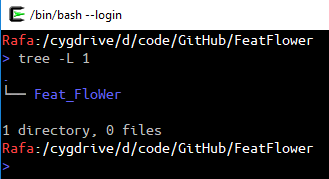
\includegraphics[width=10.0cm]{folder1.png}
  \end{center}
  \caption{Directory structure after cloning the source repository}
  \label{fig:folder1}
\end{figure}
%%%%%%%%%%%%%%%%%%%%%%%%%%%%%%%%%%%%%%%%%%%%%%%%%%%%%%%%%%%%%%%%%%%%%%%%%%%%%%%%%%%%%%%%%%%%%%%%%%%
%%%%%%%%%%%%%%%%%%%%%%%%%%%%%%%%%%%%%%%%%%%%%%%%%%%%%%%%%%%%%%%%%%%%%%%%%%%%%%%%%%%%%%%%%%%%%%%%%%%
\section{Checking out Mesh Repository}\label{mesh-repo}
As we said, the meshes are stored in a separate git repository that can be cloned by the following command: \\
\cmd{git clone ssh://username@server/home/user/git/mesh\_repo.git}\\
If the above command does not complete successfully it is very likely that you do not yet have access rights to the git mesh repository. In this case please ask your administrator to grant you
the required access rights. Your folder structure should look like in fig. \ref{fig:folder2} after cloning the mesh repository:
\begin{figure}[hb]
  \begin{center}
    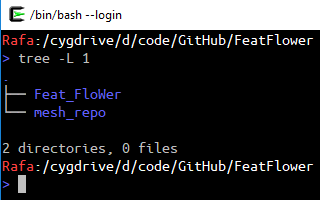
\includegraphics[width=10.0cm]{folder2.png}
  \end{center}
  \caption{Directory structure after cloning the mesh repository}
  \label{fig:folder2}
\end{figure}

\FloatBarrier
After you have checked out the mesh repository, it is time to set up an environment variable for the mesh directory. The environment variable is used during the installation of FeatFloWer, so that the mesh 
repository can be found. For the \texttt{BASH} or \texttt{ZSH} shells this can be done by adding the following line to your \textit{.bashrc} or respectively \textit{.zsh}:\\
\cmd{export Q2P1\_MESH\_DIR=/path/to/meshrepo/mesh\_repo}\\
If you are unsure how to set environment variables please learn how to set up and use environment variables in the terminal environment that you are using. Examples of shell configuration files can be found in 
section \ref{sec:shell-customization}.
%%%%%%%%%%%%%%%%%%%%%%%%%%%%%%%%%%%%%%%%%%%%%%%%%%%%%%%%%%%%%%%%%%%%%%%%%%%%%%%%%%%%%%%%%%%%%%%%%%%
\section{Building the Code from Source}\label{baz}
The FeatFloWer code can be build on Linux and Windows operating systems (and probably on MacOS, but this is not tested yet). On Linux systems an installation of the GNU compiler is needed, including the gfortran compiler and the matching OpenMPI libraries. The minimum requirement for the GCC is version 4.9.2. On Linux systems the Intel compiler can be used as an alternative compiler. On Windows systems the Intel compiler is a necessary requirement.
For Linux and derivates we recommended setting a number of environment variables and adding some customization to your shell configuration files in order to work more efficiently within the FeatFloWer framework. See section \ref{section:appendix} for more details.

\subsection{Linux Systems}
After you have cloned the repository, navigate to the \textit{FeatFlower} folder that you have created in the previous step and create another folder that will contain the binaries:\\
\cmd{mkdir bin}\\
Verify with the command \textbf{pwd} that your FeatFlower folder now contains two subfolders \textit{bin} and \textit{Feat\_FloWer}. At the core of the Feat\_FloWer build system
is the multi-platform build files generator CMake. On the servers of the TU Dortmund CMake is available as a loadable module. In order to successfully compile the code with the GNU compiler the following components are needed:
\begin{itemize}
  \item GCC the GNU Compiler Collection including the gfortran compiler
	\item A matching OpenMPI installation
	\item CMake with a minimum version of 2.8
\end{itemize}
On the servers of the TU Dortmund you need modules for the following software:
\begin{itemize}
  \item A module for a gcc version (> 4.9.2)
  \item A module for openmpi (> 2.1.5)
  \item A module for cmake (> 2.8).	
\end{itemize}
The modules on the TU Dortmund Servers are regularly updated and do undergo frequent name changes, so we do not reference specific module names here. If in doubt, ask a more experienced colleague or the 
administrator. In order for CMake to use the compiler that has been added by the module system it is recommended to set the environment variables \texttt{CC}, \texttt{CXX}, \texttt{FC} accordingly. In detail this
this means executing the commands (for \texttt{BASH} or \texttt{ZSH} shells):

\begin{itemize}
  \item \cmd{export CC=\$(which mpicc)}
  \item \cmd{export CXX=\$(which mpicxx)}
  \item \cmd{export FC=\$(which mpif90)}
\end{itemize}
for the \texttt{TCSH} or \texttt{CSH} shells use the syntax:
\begin{itemize}
  \item \cmd{setenv CC mpicc}
  \item \cmd{setenv CXX mpicxx}
  \item \cmd{setenv FC mpif90}
\end{itemize}
It is advised to create shell aliases for these commands because they are used frequently. After you have entered the load commands, verify that these module are loaded by checking the output of the command \textbf{module list}. The build of the basic software package is
initiated by navigating into the \textit{bin} folder that you have created before and evoking CMake from there:\\
\cmd{cd bin}\\
\cmd{cmake -DBUILD\_METIS=True ../Feat\_FloWer}\\
The build process is then started by the command:\\
\cmd{make -j 5}\\
The option <-j 5> starts a parallel build using 5 processes.
\subsection{Windows Systems}
Under construction
\subsection{Installation of the Partitioner}
By installing the partitioner we mean that it is configured in a way that a user can simply call it in a terminal, just as you would call any other terminal command. In order to achieve this, we set environment variables to 
the location of the necessary files in the FeatFloWer source tree, so they can be found when called and they get updated when you fetch and apply new commits from the Git repository. The required environment variables for this to work are:
\begin{itemize}
  \item \textbf{FF\_HOME}: Source directory of your FeatFloWer installation
  \item \textbf{FF\_PY\_HOME}: Source directory of the python files of your FeatFloWer installation
  \item \textbf{PATH}: Append the path to the python files to your PATH variable
  \item \textbf{LD\_LIBRARY\_PATH}: Append the path to the Metis library to your LD\_LIBRARY\_PATH variable
\end{itemize}
Instructions and examples of how to set these variables in your shell configuration can be found in Section \ref{section:appendix}.

\subsection{Using CMake-gui to build the Code}
The CMake build framework that is used to build the FeatFloWer software package comes with a GUI component. We will explain in this section how to use the GUI to build CMake from source.
\begin{figure}[hb]
  \begin{center}
    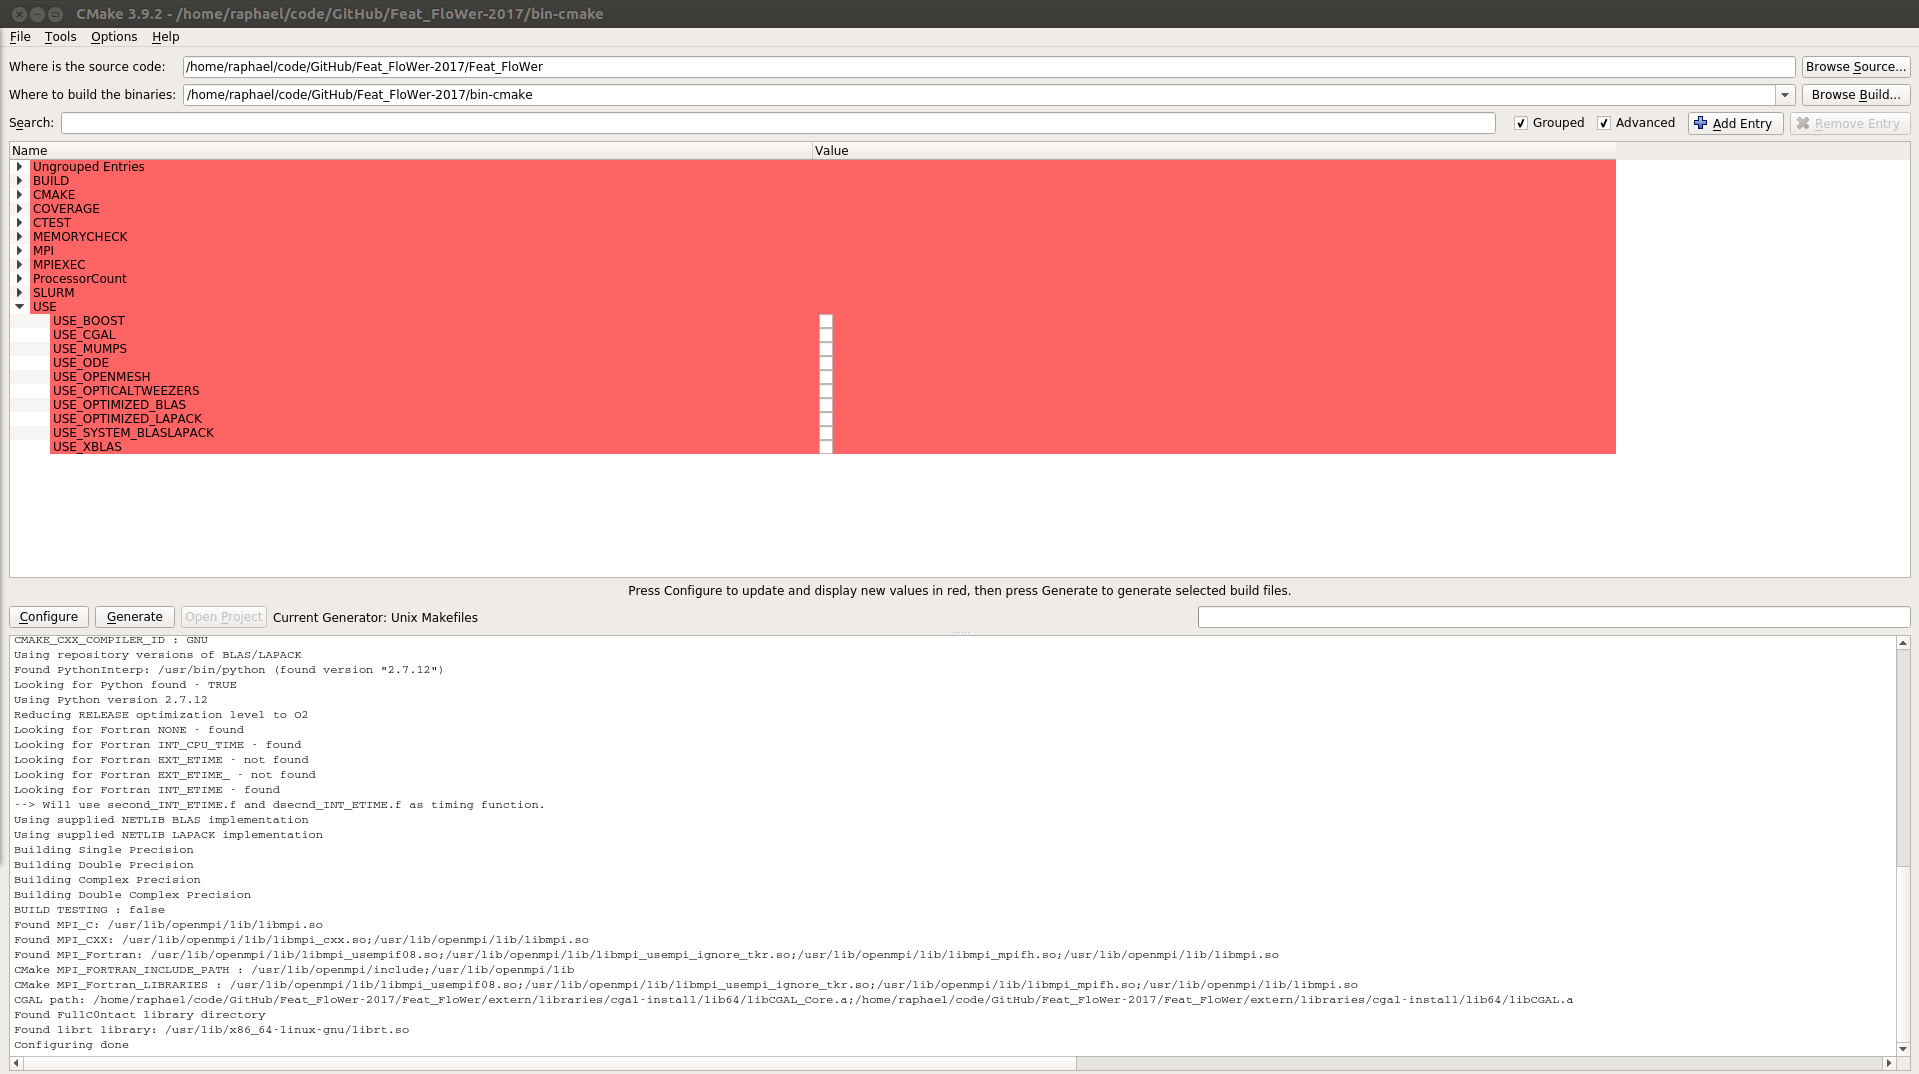
\includegraphics[width=14.5cm]{cmake-gui.png}
  \end{center}
  \caption{The CMake configuration GUI \label{fig:cmake-gui}}
\end{figure}
The main view of the CMake-gui shows you an overview of the CMake variables and their current values. Once you hit the configure button various tests are run that check for the availability of required libraries the results
of these checks are printed to the output window of the CMake GUI. If a problem occurs with the current configuration an error message is printed to the output view and usually it is descriptive enough in order to 
find and fix the configuration problem. Once there are no more configuration errors you can hit the generate button and an operating system specific build file is generated that you can use to build the code.
Additionally, the CMake-gui can give you an overview of the optional components that can be used by FeatFloWer. These optional components give the user access to extended code functionalities, solver libraries or additional simulation libraries. In the \textit{Grouped} of CMake these optional components can be found and enabled in the \textit{USE} group (see figure \ref{fig:cmake-gui}).




%%%%%%%%%%%%%%%%%%%%%%%%%%%%%%%%%%%%%%%%%%%%%%%%%%%%%%%%%%%%%%%%%%%%%%%%%%%%%%%%%%%%%%%%%%%%%%%%%%%
\chapter{Running a FeatFlower Application}
\label{ch:applications}



%%%%%%%%%%%%%%%%%%%%%%%%%%%%%%%%%%%%%%%%%%%%%%%%%%%%%%%%%%%%%%%%%%%%%%%%%%%%%%%%%%%%%%%%%%%%%%%%%%%
\section{Introduction to the Application Framework}\label{sec:introduction}
A FeatFlower application is a particular simulation case that is based on the underlying Finite-Element-Method framework. The possibility of a FeatFloWer application range from very simple CFD-Setups to well-known benchmark
configurations to complex realistic configurations that have an industrial or scientific background. The FeatFlower code base comes with a number of preconfigured applications that demonstrate the capabilities of the software. The
user can then change and adapt these preconfigured applications to his needs or add completely new applications based on the Featflower framework. A FeatFloWer applications roughly consists of a preprocessing step, a solving procedure and an output of the solution. At first we will introduce the tools used in the preprocessing step. 
\subsection{Preprocessing and Mesh Generation}
The main task in the preprocessing step is the creation of the mesh used for the FeatFloWer application. A mesh can be acquired by an external mesh generator, by manual construction or by taking a 
mesh from the FeatFloWer mesh repository. Before a mesh can be used in a parallel simulation it needs to be decomposed or partitioned so that the mpi processes can handle individual parts of the domain
in parallel. In FeatFloWer the Metis library is used to partition a mesh into submeshes. The functionality of the Metis library is accessed by a set of Python scripts that is distributed with 
FeatFloWer. We will now show how to prepare a mesh from the mesh repository for use in a parallel simulation. 
\subsubsection{Mesh Decomposition using the Python Partitioner}
In order to start a simulation we need a mesh at first, taking a mesh from the mesh repository is the easiest scenario for a new user. 
Usually this means that a benchmark configuration or a preconfigured application is run by the user. All the user has to 
do in this case is to partition the mesh according to the number of MPI processes that the user has to his disposal. The preferred partitioning tool for meshes from the mesh repository is the Python 
command line program \textit{PyPartitioner.py}. In order to demonstrate the use of the python partitioning tool, we will use the application \textit{q2p1\_fc\_ext}. The application can be found in 
the \textit{Feat\_FloWer/applications} directory. The python partitioner tool can be found in the \textit{Feat\_FloWer/tools} directory. For our first contact with the tool, we will just copy 
the python files from the \textit{Feat\_FloWer/tools} directory to the \textit{bin/applications/q2p1\_fc\_ext}. So start by navigating to the \textit{bin/applications/q2p1\_fc\_ext} and copying the 
python files by:\\
\cmd{cp ../../../Feat\_FloWer/tools/*.py .}\\
Additionally, we need to copy the metis library so that the PyPartitioner can interface with that library:\\
\cmd{cp ../../../bin/extern/libraries/metis-4.0.3/Lib/libmetis.so .}\\
We can now invoke the PyPartitioner by typing:\\
\cmd{python PyPartitioner.py 4 1 1 NEWFAC \_adc/2D\_FAC/2Dbench.prj}\\
which will take the mesh referenced in the project file \textit{\_adc/2D\_FAC/2Dbench.prj} and decompose the domain into 4 partitions which are then stored in the \textit{NEWFAC} directory. 
The additional 1 1 parameters denote the type of the partitioning method. You have now created a set of partitioned mesh files that are located in the NEWFAC directory that can by used in 
a simulation with 4+1 processes. The syntax 4+1 refers to a setup with 1 master node and 4 slave nodes. You are now ready to run the application.
\subsection{Running the Application}
As we said before, the simulation requires a master node to control some the slave processes, so the simulation should be launched with 4+1 processes by:\\
\cmd{mpirun -np 5 ./q2p1\_fc\_ext}\\
When you start a FeatFloWer application you will see the simulation output on your terminal. Additionally, the simulation output will be stored in a log or protocol file that can be found 
in the working directory of the particular application you are running under the path \textit{\_data/prot.txt}.
\subsection{Application Output and Postprocessing}
As we have mentioned the output of the simulation can be seen on the command line and in the protocol file. Detailed information such as the velocity or pressure fields of the solution 
are stored in files that are located in the \textit{\_vtk/} folder in your application working directory. The files are stored in the \textit{VTK}-format so they can be opened in our 
preferred postprocessing software \textit{ParaView}.
%%%%%%%%%%%%%%%%%%%%%%%%%%%%%%%%%%%%%%%%%%%%%%%%%%%%%%%%%%%%%%%%%%%%%%%%%%%%%%%%%%%%%%%%%%%%%%%%%%%
%%%%%%%%%%%%%%%%%%%%%%%%%%%%%%%%%%%%%%%%%%%%%%%%%%%%%%%%%%%%%%%%%%%%%%%%%%%%%%%%%%%%%%%%%%%%%%%%%%%
\section{q2p1\_cc ({\it by R. Jendrny})}

\subsection{Systems that can be solved}
Using this application you can solve the following systems in a coupled way:
\begin{itemize}
\item Stationary (Navier-) Stokes equations
\begin{align*}
\begin{pmatrix} L+K(u) & B \\ B^T & 0 \end{pmatrix} \begin{pmatrix} u \\ p \end{pmatrix} &= \begin{pmatrix} g \\ 0 \end{pmatrix},\\
\text{with } K(v) w &\sim v \cdot \nabla w.
\end{align*}
In a defect-correction procedure it is written as:
\begin{align*}
\begin{bmatrix} u^n \\ p^n \end{bmatrix} = \begin{bmatrix} u^{n-1} \\ p^{n-1} \end{bmatrix} +  \begin{bmatrix} L+R(u^{n-1}) & B \\ B^T & 0 \end{bmatrix}^{-1} &\left( \begin{bmatrix} g \\ 0 \end{bmatrix} - \begin{bmatrix} L+K(u^{n-1}) & B \\ B^T & 0 \end{bmatrix} \begin{bmatrix} u^{n-1} \\ p^{n-1} \end{bmatrix}\right) \\
\text{with } R(u^{n-1}) &= K(u^{n-1}) + \alpha \bar{M}(u^{n-1}).
\end{align*}
Changing the value $\alpha$ you can switch between Fixpoint and Newton method. If $\alpha$ = 0 the pure Fixpoint method will be used. If $\alpha \ne$ 0 the code uses an adaptive technique to switch between both methods.
\item unsteady (Navier-) Stokes equations
\begin{itemize}
\item general $\theta$-scheme
\begin{equation*}
\begin{pmatrix} M+\theta\Delta t \{L+  K(u^{n+1})\} & \Delta t B \\ B^T & 0 \end{pmatrix} \begin{pmatrix} u^{n+1} \\ p^{n+1} \end{pmatrix} = \begin{pmatrix} M u^n - (1-\theta)\Delta t \{L+K(u^n)\} u^n  \\ 0 \end{pmatrix}
\end{equation*}
\item Backward Difference Formula (BDF)
\begin{itemize}
\item BDF(1): Backward Euler method is the same.
\item BDF(2):
\begin{equation*}
\begin{pmatrix} M+\frac{2}{3}\Delta t \{L+K(u^{n+1})\} & \frac{2}{3}\Delta t B \\ B^T & 0 \end{pmatrix} \begin{pmatrix} u^{n+1} \\ p^{n+1} \end{pmatrix} = \begin{pmatrix} \frac{4}{3}M u^n - \frac{1}{3}M u^{n-1} \\ 0 \end{pmatrix}
\end{equation*}
\item BDF(3):
\begin{equation*}
\begin{pmatrix} M+\frac{6}{11}\Delta t \{L+K(u^{n+1})\} & \frac{6}{11}\Delta t B \\ B^T & 0 \end{pmatrix} \begin{pmatrix} u^{n+1} \\ p^{n+1} \end{pmatrix} = \begin{pmatrix} \frac{18}{11}M u^n - \frac{9}{11}M u^{n-1} + \frac{2}{11}M u^{n-2} \\ 0 \end{pmatrix}
\end{equation*}
\end{itemize}
\end{itemize}
\end{itemize}



\subsection{q2p1\_param.dat}
In this parameter file you have to set up all simulation parameters. Since this is a special case of the general program only the differences are listed:
\begin{itemize}
\item SimPar@TimeScheme: Choose between BE, CN (or FE); for stationary simulations this has to be BE.
\item SimPar@TimeStep: any; for stationary this has to be 1d0.
\item SimPar@MaxNumStep: Number of maximum time iterations; for stationary this has to be 1.
\item SimPar@MatrixRenewal: Only M, K and S are active in this version; for Stokes K0.
\item SimPar@FlowType: nonNewtonian is the only case that is working.
\item SimPar@SteadyState: Choose between Yes or No; for stationary this has to be Yes and in SimPar@MatrixRenewal set M to 1.
\item CCuvwp@NLmin: One possible choice is 1.
\item CCuvwp@NLmax: Maximum of non-linear iteration in each time step; for Stokes this has to be 1.
\item CCuvwp@Alpha: In general this is a value between 0d0 (Fixpoint) and 1d0 (Newton); for Stokes it is useful to take a big value (e.g. 11 which results in 1E-12 as the stopping)
\item CCuvw@ValAdap: Insert two values for the adaptivity curve (1st greater than 1, 2nd lower than 0.9): Scaling factors for the adaptivity bewtween Fixpoint and Newton
\item CCuvwp@Stopping: Relative stopping criterion for each time-step.
\item CCuvwp@MGMinLev or MGMedLev: Set this as the value of SimPar@MaxMeshLevel and the linear equations are solved by MUMPS.
\item CCuvwp@Vanka: Only 0 is working correctly.
\item CCuvwp@BDF: Choose between 0 (for BE/CN or stationary), 2 (for BDF(2)) or 3 (for BDF(3)).
\item Prop@PowerLawExp: Together with S in SimPar@MatrixRenewal the value 1.00d0 results in a Newtonian flow
\end{itemize}

\subsection{Source files}
\subsubsection*{q2p1\_cc.f90} 
This is the main routine in which the application is configured: The application gets initialized, reads all parameters, runs the simulation and does some post-processing. You can also find the time loop in this file. The initialization for all time-schemes is added compared to the first initial version.

\subsubsection*{app\_init.f90} 
It is called by the main routine, initializes the parallel structures, prepares the mesh (via decomposing the mesh to subdomains) and reads the simulation parameters SimPar. Here old solutions from older simulations can be read in, too.

\subsubsection*{assemblies\_cc.f}
Two important files are included in this file: On the one hand there is the subroutine CC\_GetDefect\_sub and on the other hand the subroutine CC\_Extraction\_sub. Both are called in the file q2p1\_def\_cc.f90 and will be explained in this file.\\
There is a subroutine which calculates the acting forces, too. But this is an old version because it is not of iso-parametric style.

\subsubsection*{iso\_assemblies.f} 
In this file all the iso-parametric stuff is included: You can find iso-parametric assemblies of the matrices M, barM, K, S (and its further components), D (which is useless at the moment) and B. Additionally, there is the iso-parametric calculation of the forces (GetForceCyl\_cc\_iso). Here the acting forces are saved as follows: The first three entries are the components of the drag, the next three entries are the components of the lift and the last entry is the force in z-direction. The components of the drag and lift are sorted. First you have the complete force, then you see the velocity component and finally there is the pressure component of the acting force. The sum of the velocity and the pressure part is the complete force. If you compare the components of each force with a reference one the sum of the component errors can be greater thant the error of the complete one since the triangular inequality holds.

\subsubsection*{lin\_transport\_cc.f90} 
???

\subsubsection*{postprocessing.f90} 
It provides some helpful subroutines. Firstly, it writes the soultion to a vtk or gmv file. Secondly, the solver statistics are output at the end of the simulation. Finally, there are routines that are important for the dump files: Some files are necessary to read old dump files and some needs to be called to write dump-files. At the moment you can choose between prf and dmp files: prf needs a lot of memory and dmp outputs the solution of all ids to one file for velocity or pressure. The code is adjusted to use dmp files at the moment.

\subsubsection*{q2p1\_cc\_Umfpacksolver.f90} 
Some files are needed for factorization of the coarse and element matrices. Since MUMPS is set as the coarse grid solver the solver routins of UMFPACK can be useless.

\subsubsection*{q2p1\_def\_cc.f90} 
Creating the system matrices and working with these is one of the main tasks in this file. At the strat the system matrices are created: You have a big block matrix $A$ for the non-linear equations and to compute the defect and a block matrix $AA$ to perform the Preconditioner, i.e. $x^n = x^{n-1} + AA^{-1}(b-A x^{n-1}$. The block matrices will only work with S (D is not working; but with S you can simulate Newtonian fluids as well.). In the bottom of this file all matriy assemblies are called to create these using the iso-parametric concept.\\
In this file you can find some more basic routines that are important for the CC code: One of them calculates the defect (using CC\_GetDefect\_sub) and the next calculates the norm of this (non-linear) defect. \\
Of course, there are routines which are special for the CC version. There is a subroutine which creates special CC structures. These structures are used by CC\_Extraction and Special\_CC\_Coarse. Without these two subroutines the code uses wrong matrices in the solver and you will get wrong results.\\ 
Ultimately the MG solver is initilaized and called in CC\_mgSolve.

\subsubsection*{q2p1\_mg\_cc.f90} 
??

\subsubsection*{q2p1\_transport\_cc.f90} 
Before the main working subroutine is implemented some structures for the CC solver are initialized.\\
The main working/solving routine is Transport\_q2p1\_UxyzP\_cc. The following sketch will show how this routins is working:
\begin{itemize}
\item Generate the adaptive function to have a background how to switch between Fixpoint and Newton method.
\item Assemble the right hand side.
\item Regarding time schemes set the correct scaling factor.
\item Assemble the system matrices
\item Factorize the element matrices.
\item Compute the initial defect.
\item Call the MG solver.
\item Perform a full update of the solution
\item Depending on the change of the defects the code decides if it can endure more Newton influence or less. The scaling is influenced by the adaptive function.
\item Depending on the change of the defects and the use of Newton or Fixpoint the stopping criterion for MG is changed.
\item Calculate the acting forces.
\item Does the solution fulfill the non-linear stopping criterion?
\end{itemize}
In this file you can also find two subroutines which calculate the acting forces: On the one hand FAC\_GetForces\_CC\_iso that is calling GetForceCyl\_cc\_iso and is the default decision; on the other hand there is a subroutine that calculates the forces using $S u + Bp$ (myFAC\_GetForces).\\
The last important subroutine reads the CCuvwp parameters which are set in the param file.

\subsubsection*{q2p1\_var\_newton.f90} 
Additionally to QuadSc\_var.f90 you can find a few new variables:
\begin{itemize}
\item Variables for the Newton-Preconditioner: barMXYmat, mg\_barMXYmat, AAXYmat and mg\_AAXYmat,
\item variables for the force calculation using myFAC\_GetForces: BXMat\_new, mg\_BXMat\_new (Since the general B matrices are influenced by the Dirichlet BC there was a need to have B matrices without these BC to have correct forces.),
\item a new type for the CC parameters used in the param.dat: TYPE tParamCC and
\item additional variables for the BDF schemes
\end{itemize}

\subsection{How to compile and run the code}
The following comments compile the code and run it:\\
{\scriptsize\cmd{cmake -DQ2P1\_BUILD\_ID=xeon-linux-intel-release -DBUILD\_APPLICATIONS=True -DUSE\_MUMPS=True ../Feat\_FloWer/}}\\
\cmd{make -j4}\\
\cmd{PyPartitioner.py 8 1 1 NEWFAC 'FILE.prj'}\\
\cmd{mpirun -np 9 ./q2p1\_cc}\\


%%%%%%%%%%%%%%%%%%%%%%%%%%%%%%%%%%%%%%%%%%%%%%%%%%%%%%%%%%%%%%%%%%%%%%%%%%%%%%%%%%%%%%%%%%%%%%%%%%%
%%%%%%%%%%%%%%%%%%%%%%%%%%%%%%%%%%%%%%%%%%%%%%%%%%%%%%%%%%%%%%%%%%%%%%%%%%%%%%%%%%%%%%%%%%%%%%%%%%%
\section{Appendix}\label{section:appendix}
\textbf{TODO}

\subsection{Recommended Shell Customizations For Linux Systems}
\label{sec:shell-customization}
In order to work more efficiently with the FeatFloWer software, we recommended to add some environment variables and aliases 
to your shell configuration files in order to make your experience with the software more pleasant. Sample configuration files are provided in the FeatFloWe repository you have cloned in the
first steps. The configuration files can be found in the repository under the following path:
\cmd{/path/to/Feat\_FloWer/tools/shell\_scripts/featflower\_scripts}\\
There sample configuration for different shells can be found. As can be seen in the following listings, the configuration files contain aliases for loading compiler settings, customizations for 
the command line for the Git version control system and setting environment variables so that the different FeatFloWer auxilliary scripts are contained in the path and can be easily called from the
command line.
\subsubsection*{TCSH and CSH} 

\begin{Verbatim}[numbers=left, frame=single, label=TCSH]
#!/bin/csh

set prompt = "%B%m%b:%~%# "

#========================================================
#        Environment variables for Feat_FloWer
#========================================================
# Adjust these paths to point them to the directories of
# your local installation.
setenv Q2P1_MESH_DIR /path/to/mesh_repo
setenv FF_HOME /path/to/Feat_FloWer
setenv FF_PY_HOME /path/to/Feat_FloWer/tools

#========================================================
#                  GCC Aliases
#========================================================
alias load-gcc-mpi51 'module purge ;; \
module load cmake/3.5.2 \
gcc/5.1.0 \
openmpi/gcc5.1.x/1.10.2/threaded/no-cuda/ethernet \
boost/1.56 python/2.7.11 ;; \
setenv CC mpicc ;; setenv CXX mpicxx ;; setenv FC mpif90'

alias load-gcc-mpi61 'module purge ;;\
module load cmake/3.4.0 \
gcc/6.1.0 \
openmpi/gcc6.1.x/1.10.2/non-threaded/no-cuda/ethernet \
boost/1.56 python/2.7.11 ;; \ 
setenv CC mpicc ;; setenv CXX mpicxx ;; setenv FC mpif90'

#========================================================
#               Intel Compiler Aliases
#========================================================
alias load-intel-mpi16 'module purge ;; \
module load cmake/3.5.2-ssl \ 
intel/studio-xe/16.0.4.258 \
openmpi/intel16.0.x/1.8.8/non-threaded/no-cuda/ethernet \
gcc/6.1.0 boost/1.56 python/2.7.11 ;; \
setenv CC mpicc ;; \
setenv CXX mpicxx ;; \
setenv FC mpif90'


#========================================================
#               Library Path for Metis
#========================================================
setenv LD_LIBRARY_PATH \
      $LD_LIBRARY_PATH:/path/to/metis-4.0.3/Lib


#========================================================
#        Customization for Git Version Control
#========================================================
source ~/autocompletion.tcsh

#git completion
source ~/.git-completion.tcsh

# set prompt; with current git branch if available.
alias __git_current_branch \

'git rev-parse --abbrev-ref HEAD >& /dev/null && \
echo "{`git rev-parse --abbrev-ref HEAD`}"'

alias precmd \
'set prompt="%n@%m[%c2]`__git_current_branch` "'

#========================================================
#                 PATH Variable
#========================================================
# Do further customization of your PATH here:
setenv PATH $PATH:/path/to/Feat_FloWer/tools/partitioner

module purge ;; module load gcc/6.1.0 \
openmpi/gcc6.1.x/1.10.2/non-threaded/no-cuda/ethernet \
cmake 

setenv CC mpicc
setenv CXX mpicxx
setenv FC mpif90
\end{Verbatim}

\subsubsection*{BASH and ZSH} 

\begin{Verbatim}[numbers=left, frame=single, label=BASH]
#!/bin/bash
#========================================================
#Author: Raphael Muenster
#This script automizes module loading
#and console environment configuration
#========================================================


# Uncomment this line and assign a value to the EDITOR
# variable to set your default editor.
#export EDITOR=

#========================================================
#         Environment variables for Feat_FloWer
#========================================================
# Adjust these paths to point them to the directories 
# of your local installation.

export Q2P1_MESH_DIR=/path/to/mesh_repo
export FF_HOME= /path/to/Feat_FloWer
export FF_PY_HOME=/path/to/Feat_FloWer/tools
export PATH=$PATH:/path/to/Feat_FloWer/tools/partitioner

#========================================================
#                    Cluster Logins
#========================================================
alias ssh-lido='ssh username@lidong1.itmc.tu-dortmund.de\
  -L 11111:lidong1.itmc.tu-dortmund.de:11111'
alias ssh-lido3='ssh username@gw02.lido.tu-dortmund.de\
  -L 11111:gw02.lido.tu-dortmund.de:11111'

#========================================================
#                  TMUX Configuration
#========================================================
# Set the screen variable of the tmux terminal multiplexer
alias tmux="TERM=screen-256color-bce tmux"

#========================================================
#               Intel Compiler Aliases
#========================================================
alias load-intel-mpi15='module purge && module load \ 
intel/studio-xe/15.0.7.235 gcc/5.4.0 boost/1.56 \
openmpi/intel15.0.x/1.10.2/non-threaded/no-cuda/ethernet \
cmake && export CC=mpicc && export CXX=mpicxx &&  \
export FC=mpif90'
alias load-intel-mpi16='module purge && module load \ 
intel/studio-xe/16.0.4.258 binutils/2.25 \
gcc/6.1.0 \
openmpi/intel16.0.x/1.8.8/non-threaded/no-cuda/ethernet \
cmake && export CC=mpicc && export CXX=mpicxx && \
export FC=mpif90'

#========================================================
#                     GCC Aliases
#========================================================
alias load-gcc-mpi61='module purge && module load cmake \
gcc/6.1.0 boost/1.56 \
openmpi/gcc6.1.x/1.10.2/non-threaded/no-cuda/ethernet \
&& export CC=$(which mpicc) && \ 
export CXX=$(which mpicxx) && export FC=$(which mpif90)'

#========================================================
#                    PATH Variable
#========================================================
# Do further customization of your PATH here:
#export PATH=$PATH:$HOME/nobackup/bin 

#========================================================
#                 Library Path for Metis
#========================================================
export LD_LIBRARY_PATH=$LD_LIBRARY_PATH: \
/path/to/metis-4.0.3/Lib

module purge && module load gcc/6.1.0 && \ 
module load \ 
openmpi/gcc6.1.x/1.10.2/non-threaded/no-cuda/ethernet \
&& module load cmake && export CC=mpicc && \
export CXX=mpicxx && export FC=mpif90

\end{Verbatim}

%%%%%%%%%%%%%%%%%%%%%%%%%%%%%%%%%%%%%%%%%%%%%%%%%%%%%%%%%%%%%%%%%%%%%%%%%%%%%%%%
\end{document}

